\documentclass[9pt]{beamer}

%~~~~~~~~~~~~~~~~~~~~~~~~~~~~~~~~~~~~~~~~~~~~~~~~~~~~~~~~~~~~~~~~~~~~~~~~~~~~~~
\usepackage[sfdefault]{roboto}
\usepackage[utf8]{inputenc}
\usepackage[T1]{fontenc}
%~~~~~~~~~~~~~~~~~~~~~~~~~~~~~~~~~~~~~~~~~~~~~~~~~~~~~~~~~~~~~~~~~~~~~~~~~~~~~~

%~~~~~~~~~~~~~~~~~~~~~~~~~~~~~~~~~~~~~~~~~~~~~~~~~~~~~~~~~~~~~~~~~~~~~~~~~~~~~~
\usepackage{styles/fluxmacros}
\usefolder{styles}
\usetheme[style=lila]{flux}
%~~~~~~~~~~~~~~~~~~~~~~~~~~~~~~~~~~~~~~~~~~~~~~~~~~~~~~~~~~~~~~~~~~~~~~~~~~~~~~

%~~~~~~~~~~~~~~~~~~~~~~~~~~~~~~~~~~~~~~~~~~~~~~~~~~~~~~~~~~~~~~~~~~~~~~~~~~~~~~
% Extra packages for the demo:
\usepackage{booktabs}
\usepackage{colortbl}
\usepackage{ragged2e}
\usepackage{schemabloc}
\usepackage{graphicx}
\usepackage{lastpage}
%~~~~~~~~~~~~~~~~~~~~~~~~~~~~~~~~~~~~~~~~~~~~~~~~~~~~~~~~~~~~~~~~~~~~~~~~~~~~~~

%~~~~~~~~~~~~~~~~~~~~~~~~~~~~~~~~~~~~~~~~~~~~~~~~~~~~~~~~~~~~~~~~~~~~~~~~~~~~~~
% Informations
\title{
	\fontsize{13}{15}\selectfont Prinzipien und Anwendung des Softwaredesigns \\[5px] 
	\textbf{\color{primary} \fontsize{11}{13}\selectfont anhand von Schichten- und Hexagonaler Architektur} 
}
\author{Simon Thalmaier}
\institute{Informatik Bachelor}
\date{\today}
\titlegraphic{assets/thi.png}
%~~~~~~~~~~~~~~~~~~~~~~~~~~~~~~~~~~~~~~~~~~~~~~~~~~~~~~~~~~~~~~~~~~~~~~~~~~~~~~

\def\footerimage{assets/Progress.png}
\def\numbersofframe{6}

\begin{document}

% Generate title page
\titlepage


\begin{frame}[noframenumbering]
 \frametitle{Software Design}
 
 Qualitätseigenschaften von Software: \\[0.5cm]
 
 \setblockstyle{native} % Default behavior, optional line.
 \begin{minipage}[b]{0.5\textwidth}
 	
 	\begin{itemize}
 		\item \alert{Zuverlässigkeit}
 		\item \alert{Effizienz}
 		\item \alert{Erweiterbarkeit}
 		\item \alert{Sicherheit}
 		\item \alert{Skalierbarkeit}
 		\item \alert{Testbarkeit}  
 	\end{itemize}
 	
 \end{minipage}
 \\[1cm]
 Um diese Eigenschaften zu stärken können gängige Architekturen und Design-Prinzipien implementiert werden.
 
\end{frame}

\def\footerimage{assets/Progress2.png}
\begin{frame}
	\frametitle{SOLID-Prinzipien}
	
	Das SOLID-Akronym beinhaltet fünf Prinzipien: \\[0.5cm]
	
	\setblockstyle{native} % Default behavior, optional line.
	\begin{minipage}[b]{0.5\textwidth}
		
		\begin{itemize}
			\item \alert{Single-Responsibility-Prinzip}
			\item \alert{Open-Closed-Prinzip}
			\item \alert{Liskovsches Substitutionsprinzip}
			\item \alert{Interface-Segregation-Prinzip}
			\item \alert{Dependency-Inversion-Prinzip}
		\end{itemize}
		
	\end{minipage}
	\\[1cm]
	
\end{frame}

\def\footerimage{assets/Progress3.png}
\begin{frame}
	\frametitle{Schichtenarchitektur}
	
	\begin{center}
		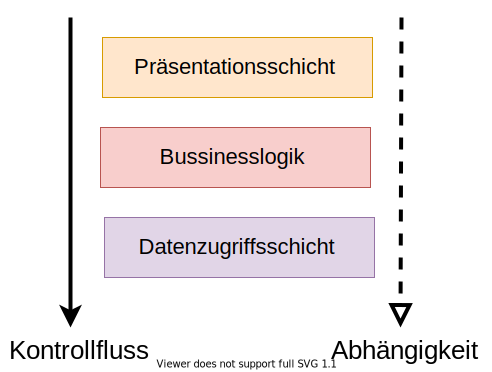
\includegraphics[width=0.7\linewidth]{assets/Schichtenarchitektur.png}
	\end{center}
	
\end{frame}

\def\footerimage{assets/Progress4.png}
\begin{frame}
	\frametitle{Hexagonale Architektur}
	
	\begin{center}
		\includegraphics[width=0.65\linewidth]{assets/HexagonaleArchitektur.png}
	\end{center}
	
\end{frame}

\def\footerimage{assets/Progress5.png}
\begin{frame}
	\frametitle{Bewertung}
	
	\textbf{\color{primary} Schichtenarchitektur \hspace{2.5cm} Hexagonale Architektur }  \\[0.2cm]
	\includegraphics[width=\linewidth]{assets/Bewertung.png}
	
\end{frame}

\begin{frame}
	\frametitle{Abschluss}
	
	\centering
	\Huge Haben Sie noch Fragen?
	
\end{frame}

\end{document}